\RequirePackage{scrlfile}
\makeatletter
\AfterPackage{beamerbasemodes}{\beamer@amssymbfalse}
\makeatother

\documentclass{beamer}
\usetheme{Darmstadt}
\usepackage{amsmath, amssymb, mathtools, tipa, tikz, kotex}
\usepackage{fancyvrb} % to frame verbatim environment
\usepackage[charter,cal=cmcal]{mathdesign}
\usepackage{relsize}
\usepackage{graphicx}
\usepackage{xcolor}
\usepackage{tcolorbox}
\usepackage{framed}
\usepackage{soul}
\renewcommand{\sfdefault}{\rmdefault}
\usepackage[T1]{fontenc}
\usefonttheme{professionalfonts} % default family is serif
\beamertemplatenavigationsymbolsempty % remove navigation bar
\newcommand{\ipa}{\textipa}
\newcommand{\ttt}[1]{\texttt{#1}}
\newcommand{\mcal}[1]{\mathcal{#1}}
\newcommand{\mbb}[1]{\mathbb{#1}}
\newcommand{\mbf}[1]{\mathbf{#1}}
\newcommand{\mrm}[1]{\mathrm{#1}}
\newcommand{\msf}[1]{\mathsf{#1}}
\newcommand{\mtt}[1]{\mathtt{#1}}
\newcommand{\msc}[1]{\text{\textsc{#1}}}
\renewcommand{\ul}[1]{\underline{#1}}
\renewcommand{\comment}[1]{\hfill $\triangleright$ #1}
\newcommand{\mcomment}[1]{\text{\comment{#1}}}
\renewcommand{\:}{\text{ }}
\renewcommand{\mod}{\text{ mod }}
\newcommand{\ord}[1]{\mrm{ord}_{#1}}

\definecolor{darkblue}{rgb}{0.2, 0.2, 0.7}

\title{HRP}
\subtitle{Shor's Algorithm \st{and Grover's Algorithm}}
\author{Seungwoo Han}
% \institute{Korea Science Academy}
\date{\today}

\hypersetup{
    colorlinks=false,      
    urlcolor=cyan,
    pdftitle={},
    pdfpagemode=FullScreen,
    }

\setbeamerfont{frametitle}{size=\large, series=\bfseries}

\begin{document}
    
    \begin{frame}
        \titlepage
    \end{frame}

    \section{Quantum Computing}
    \subsection{Quantum State}
    \begin{frame}{Quantum State}
        \begin{block}{Quantum State}
            Consider a quantum system with $n$ qubits, each of which can have two states---0 and 1.
            In quantum physics, the state of the quantum system is a point in a $2^n$-dimensional vector space.\\[1em]
            If we let $\vert S_i \rangle$\footnote{\textit{ket} notation} to denote basis vectors (or \alert{pure states}) where $i$ ranges from $0$ to $2^n-1$,
            a state, or a \alert{superposition} of the states, is represented by \\[.7em]
            \centerline{$\displaystyle \sum_{i=0}^{2^n-1} a_i \,\vert S_i \rangle$}\vspace*{.7em}
            where $a_i \in \mbb{C}$ and $\sum_{i=0}^{2^n-1} |a_i|^2 = 1$.
        \end{block}
    \end{frame}

    \begin{frame}{Probability of Being Observed}
        \begin{block}{Observation}
            If the machine is observed (w.r.t. the basis), the \alert{probability of seeing the state} $\vert S_i \rangle$ is $|a_i|^2$.\\[1em]
            We are not going to explore deeply regarding how quantums work in real life, but we shall focus on the mathematical part of quantum system.
        \end{block}
        \begin{alertblock}{}
            Since multiplying by a unit-length complex number does not change the behavior of a state,
            $2^n-1$ number of complex numbers are enough to completely describe a state.
        \end{alertblock}
    \end{frame}

    \subsection{Mathematical Background}
    \begin{frame}{Hermitian Conjugate}
        \begin{exampleblock}{Hermitian Conjugate}
            For $A \in \mrm{Mat}_{m \times n}(\mbb{C})$, the \alert{Hermitian conjugate} of $A$, denoted by $A^\ast$($\in \mrm{Mat}_{n \times m}(\mbb{C})$), is defined by
            \[ A^\ast = \overline{A}^\mrm{T} = (\overline{a_{ji}}) \]
            where $a_{ij}$ denotes the $(i, j)$ entry of $A$.
        \end{exampleblock}
    \end{frame}

    \begin{frame}{Inner Product and Norm}
        \begin{exampleblock}{Standard Inner Product}
            For $\mbf{u}, \mbf{v} \in \mbb{C}^n$, which are both column vectors in a $n$-dimensional complex vector space,
            the standard inner product is
            \[ \langle \mbf{u}, \mbf{v} \rangle = \mbf{v}^\ast \mbf{u}\text{.} \]
            Note that $\langle \mbf{u}, \mbf{v} \rangle \in \mbb{C}$.
        \end{exampleblock}
        \begin{exampleblock}{Norm}
            For $\mbf{v} = (v_1, v_2, \cdots, v_n) \in \mbb{C}^n$,
            \[ \Vert \mbf{v} \Vert^2 \triangleq \langle \mbf{v}, \mbf{v} \rangle = \sum_{i=1}^n |v_i|^2\text{.} \]
        \end{exampleblock}
    \end{frame}

    \begin{frame}{Unitary Matrix}
        \begin{exampleblock}{Unitary Matrix}
            For $A \in \mrm{Mat}_{n \times n}(\mbb{C})$, $A$ is \alert{unitary} if $A^\ast = A^{-1}$, i.e.,
            \[ A A^\ast = A^\ast A = I_n\text{,} \]
            where $I_n$ is the $n \times n$ identity matrix.
        \end{exampleblock}
        \begin{alertblock}{}
            For $\mbf{u}, \mbf{v} \in \mbb{C}^n$ and a unitary $A \in \mrm{Mat}_{n \times n}(\mbb{C})$,
            \[ \langle A\mbf{u}, A\mbf{v} \rangle = \mbf{v}^\ast A^\ast A \mbf{u} = \mbf{v}^\ast \mbf{u} = \langle \mbf{u}, \mbf{v} \rangle\text{.} \]
            Especially,
            \[ \Vert A\mbf{v} \Vert^2 = \langle A\mbf{v}, A\mbf{v} \rangle = \langle \mbf{v}, \mbf{v} \rangle = \Vert \mbf{v} \Vert^2 \text{.} \]
        \end{alertblock}
    \end{frame}

    \subsection{Quantum Gate}
    \begin{frame}{Changing a State to Another}
        \begin{block}{Changing a State to Another}
            In order to use a physical system for computation, we must be able to change the state of the system.
            The laws of quantum mechanics \alert{only permit unitary} transformations of state vectors.
        \end{block}
        \begin{alertblock}{Physical (or Realistic) Limitations}
            \small
            Quantum circuits (and quantum Turing machines) only allows \textit{local} unitary transformations;
            that is, unitary transformations on \alert{a fixed number of bits}.
            Two-bit transformations can at least in theory be implemented by relatively simple physical systems,
            while a general $n$-bit unitary transformation being implemented in real life seems to be in a remote future.\\
            We are not going to investigate the precise definitions of them, but we are going to use \alert{polynomially many} those two-bit local transformations.
        \end{alertblock}
    \end{frame}

    \begin{frame}{Quantum Gate}
        \begin{block}{Quantum Gate}
            A \alert{quantum gate} can be expressed as a (unitary) complex-valued matrix. For instance, a unitary matrix
            \begin{table}
                \small
                \centering
                \begin{tabular}{ccccc}
                                                            & $\vert 00 \rangle$ & $\vert 01 \rangle$ & $\vert 10 \rangle$ & $\vert 11 \rangle$                 \\
                    \multicolumn{1}{c|}{$\vert 00 \rangle$} & 1                  & 0                  & 0                  & \multicolumn{1}{c|}{0}             \\
                    \multicolumn{1}{c|}{$\vert 01 \rangle$} & 0                  & 1                  & 0                  & \multicolumn{1}{c|}{0}             \\
                    \multicolumn{1}{c|}{$\vert 10 \rangle$} & 0                  & 0                  & $1/\sqrt{2}$       & \multicolumn{1}{c|}{$1/\sqrt{2}$}  \\
                    \multicolumn{1}{c|}{$\vert 11 \rangle$} & 0                  & 0                  & $1/\sqrt{2}$       & \multicolumn{1}{c|}{$-1/\sqrt{2}$}
                \end{tabular}
            \end{table}
            corresponds to the transform
            \small
            \begin{align*}
                \vert 00 \rangle & \:\longrightarrow\: \vert 00 \rangle \\
                \vert 01 \rangle & \:\longrightarrow\: \vert 01 \rangle \\
                \vert 10 \rangle & \:\longrightarrow\: (\vert 10 \rangle + \vert 11 \rangle) / \sqrt{2} \\
                \vert 11 \rangle & \:\longrightarrow\: (\vert 10 \rangle - \vert 11 \rangle) / \sqrt{2}\text{.}
            \end{align*}
        \end{block}
    \end{frame}

    \begin{frame}{Quantum Gate Array}
        \begin{block}{Quantum Gate Array}
            A \alert{quantum gate array} is a set of quantum gates with logical ``wires'' connecting their inputs and outputs.
            % \begin{center}
            %     \begin{figure}
            %         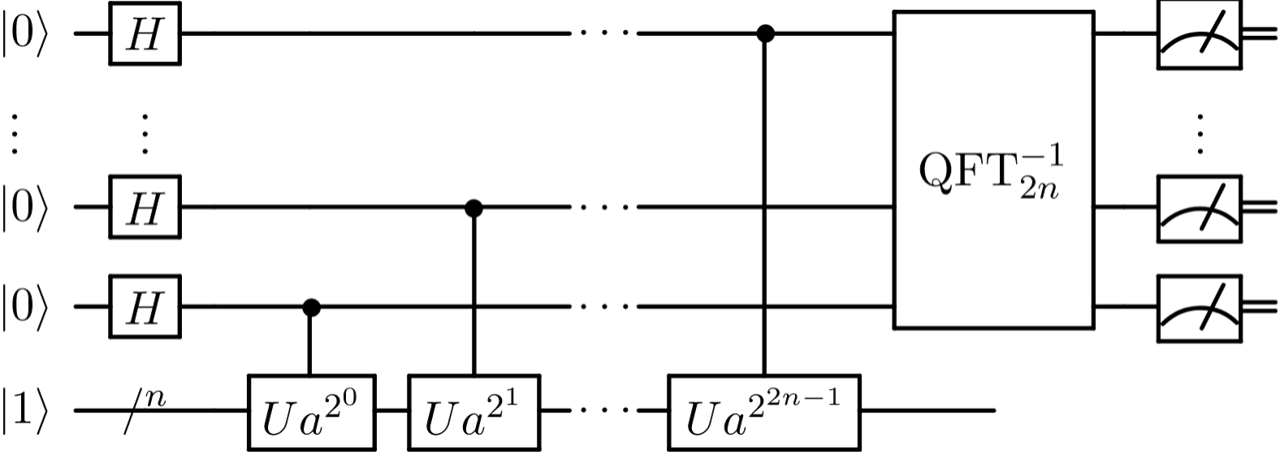
\includegraphics[width=0.4\linewidth]{shor_circuit.png}
            %     \end{figure}
            % \end{center}
        \end{block}
        \begin{alertblock}{We need to design our circuit \textit{uniformly}}
            \small
            Since there will be a different gate array for each size of input, our circuit design must be \textit{uniform}, i.e.,
            \begin{itemize}
                \setlength\itemsep{-0.2em}
                \item the design of the circuit should be produced by a polynomial-time (classical) computation and
                \item entries in the unitary matrices describing the gates must be computable numbers.\footnote{The first $\log n$ bits of each entry should be classically computable in time polynomial in $n$.}
            \end{itemize}
        \end{alertblock}
    \end{frame}

    \subsection{Revesible Computation}

    \begin{frame}{We Need Reversibility}
        \begin{alertblock}{Why do we need reversibility?}
            \small
            We have to initialize \textit{registers}\footnote{where out input-output qubits are stored} to prepare the next round of computation.
            But, manually setting registers to zero is not possible in quantum computers because \alert{superpositions of states need to be maintained} throughout the whole computation.\\
            Therefore, we need to reverse our computation only with the output, which means we shall make use of completely reversible gate arrays.
        \end{alertblock}
    \end{frame}

    \begin{frame}{Reversible Gate}
        \begin{block}{Reversible Gate}
            In \alert{reversible gates}, we can recover the input from the output.
            Most classical logic gates are irreversible; one cannot recover inputs from an output of the \ttt{NOT} gate.
        \end{block}
    \end{frame}

    \begin{frame}{Toffoli Gate}
        \begin{block}{Toffoli Gate (1980)}
            Toffoli gate\footnote{or sometimes called \ttt{CCNOT} (controlled-controlled-not) gate} is a reversible gate that is expressed as the following matrix.
            \scriptsize
            \[
                \begin{bmatrix}
                    1 & 0 & 0 & 0 & 0 & 0 & 0 & 0 \\
                    0 & 1 & 0 & 0 & 0 & 0 & 0 & 0 \\
                    0 & 0 & 1 & 0 & 0 & 0 & 0 & 0 \\
                    0 & 0 & 0 & 1 & 0 & 0 & 0 & 0 \\
                    0 & 0 & 0 & 0 & 1 & 0 & 0 & 0 \\
                    0 & 0 & 0 & 0 & 0 & 1 & 0 & 0 \\
                    0 & 0 & 0 & 0 & 0 & 0 & 0 & 1 \\
                    0 & 0 & 0 & 0 & 0 & 0 & 1 & 0 \\
                \end{bmatrix}
            \] \small
            Or simply, $(a, b, c) \mapsto (a, b, c \oplus (a \land b))$. Note that,\\[-0.2em]
            \begin{itemize}
                \setlength\itemsep{-0.2em}
                \item Toffoli gate is a reversible gate and
                \item if $c$ is fixed to 1, the third output bit is $a \:\mtt{NAND}\: b$.
            \end{itemize}
        \end{block}
        
    \end{frame}

    \begin{frame}{Classical Circuits Can Be Made Reversible}
        \begin{block}{Toffoli Gate is Universal}
            Since \ttt{NAND} gate is enough to represent all the other gates\footnote{\ttt{NOT}: $\lnot A = A \:\mtt{NAND}\: A$, \ttt{OR}: $A \lor B = \lnot (\lnot A \:\mtt{NAND}\: \lnot B)$, and so on},
            i.e., \ttt{NAND} is \textit{universal},
            it naturally follows that Toffoli gate is also universal.
        \end{block}
        \begin{alertblock}{Classical Circuits Can Be Made Reversible}
            Though it will cost a large amount of space, every classical circuit, including multiplication and modular exponentiation,
            can be converted into its reversible version (but with extra input and output bits), because Toffoli gate is both reversible and universal.
        \end{alertblock}
    \end{frame}

    \begin{frame}{Bennett's Method}
        \begin{block}{Bennett's Method (1973) \href{https://quantum-computing.ibm.com/composer/docs/iqx/guide/shors-algorithm}{\beamergotobutton{WWW}}}
            \small
            We need the input bits to be completely reset; if input bits are not reset after a round of computation, it will affect the next round.
            This is possible in reversible circuits, and one way is Bennett's method, which is described by the bottom picture,
            where\\[-0.2em]
            \begin{itemize}
                \setlength\itemsep{-0.2em}
                \item $f(x)$ is the value we want to know, and
                \item $g(x)$ is the extra output bits used to calculate $x$ from $f(x)$.
            \end{itemize} 
        \end{block}
        \begin{figure}
            \centering
            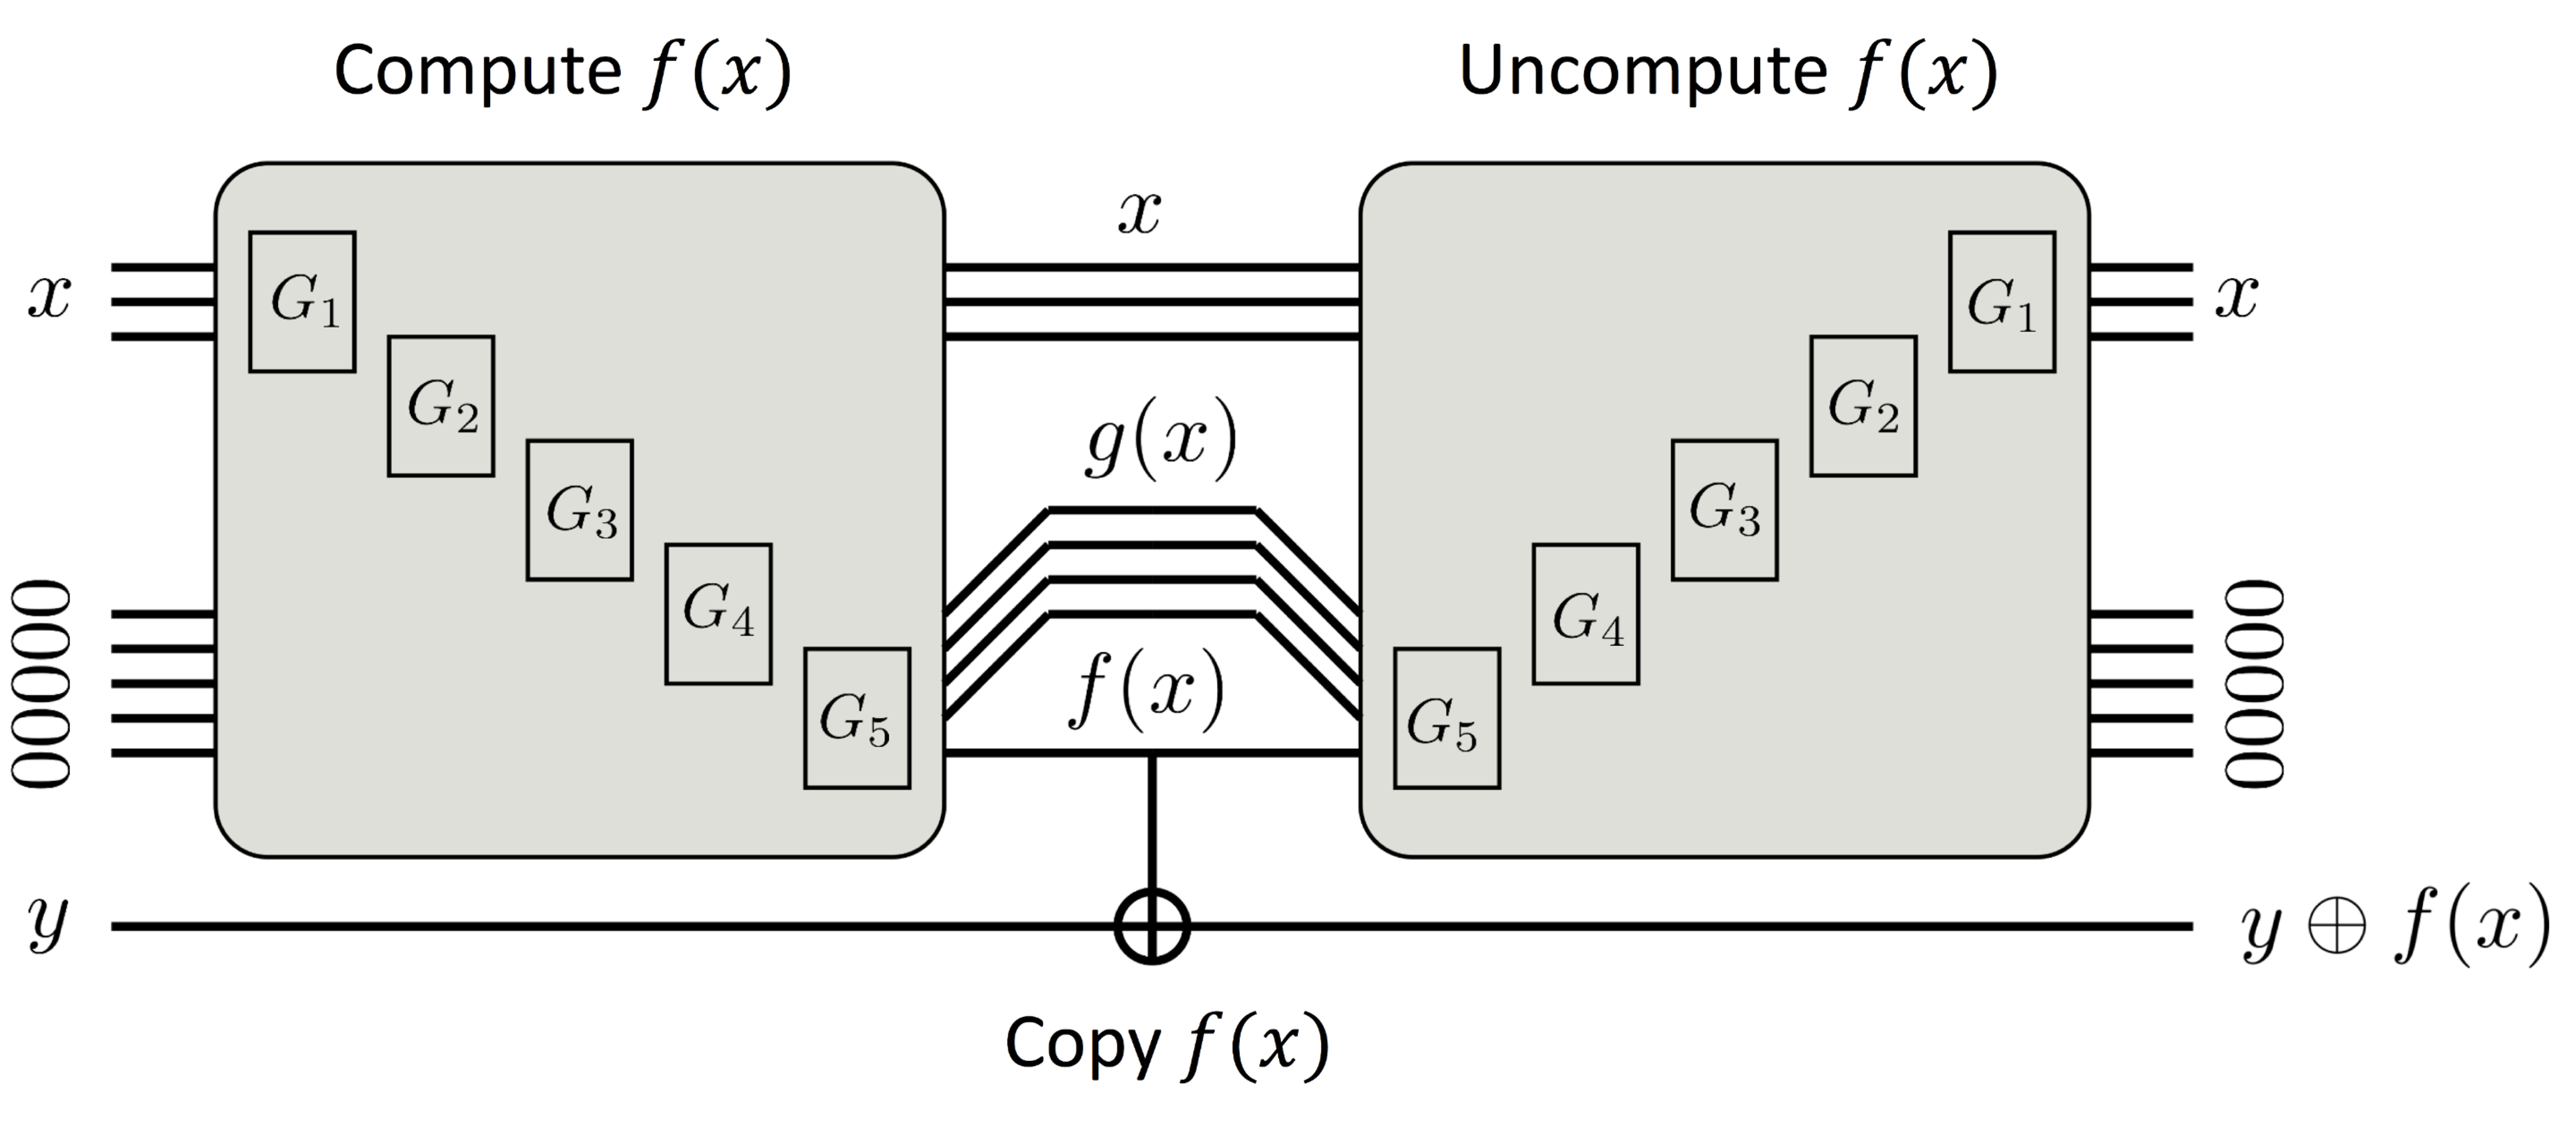
\includegraphics[width=0.7\linewidth]{bennett_method.png}
        \end{figure}
    \end{frame}

    \section{Shor's Algorithm}
    \begin{frame}
        % \begin{center}
            \begin{tcolorbox}[width=\linewidth, halign=center, colback=darkblue, boxsep=5mm, arc=3mm, boxrule=0pt]
                \centering
                \color{white} \Large
                \textbf{Shor's Algorithm} \\[1em]
                \small
                \begin{flushleft}
                    Problem $\textsc{Factoring}$:
                \end{flushleft} \vspace*{-.7em}
                Given a composite $n \in \mbb{N}$, find a non-trivial divisor $d$ of $n$.
            \end{tcolorbox}
        % \end{center}
        % \centerline{\fbox{}}
    \end{frame}

    \subsection{Mathematical Background}
    \begin{frame}{Order (Number Theory)}
        \begin{exampleblock}{}
            \begin{itemize}
                \item Given $a, b, n \in \mbb{Z}$, ``$a \equiv_n b$'' denotes ``$a \equiv b \pmod{n}$'', i.e., ``$\exists k \in \mbb{Z},\: a = b + kn$''
                \item Given $a \in \mbb{Z}$ and $n \in \mbb{N}$, ``$a \mod n$'' is the unique integer $b$ such that $0 \leq b < n$ and $a \equiv_{n} b$.
            \end{itemize}
        \end{exampleblock}
        \begin{exampleblock}{Order}
            Given $a \in \mbb{Z}$ and $n \in \mbb{N}_{>1}$ with $\gcd (a, n) = 1$,
            the \alert{order of $a$ modulo $n$}, denoted by $\ord{n} a$, is defined to be
            \[ \ord{n} a \triangleq \min \{ i \in \mbb{N} \:|\: a^i \equiv_n 1 \} \]
            The existence is guaranteed by Euler's theorem, $a^{\phi(n)} \equiv_n 1$,
            where $\phi$ is Euler's totient function.
        \end{exampleblock}
    \end{frame}

    \hypertarget{isomorphism}{
    \begin{frame}{Bijection Among $\mbb{Z}_n^\ast$s }
        Let $\mbb{Z}_n^\ast$ denote the multiplicative group of integers modulo $n$. ($|\mbb{Z}_n^\ast| = \phi(n)$)
        \begin{exampleblock}{Theorem. (variant of Chinese remainder theorem)}
            Let $n, n_1, n_2, \cdots, n_k \in \mbb{N}_{>1}$ are given where $n = \prod_{i=1}^k n_i$ and $n_i$'s are pairwise coprime.\\
            Define $f \colon \mbb{Z}_n^\ast \to \mbb{Z}_{n_1}^\ast \times \mbb{Z}_{n_2}^\ast \times \cdots \times \mbb{Z}_{n_k}^\ast$\footnote{$\times$ is Cartesian product} by\\[.4em]
            \centerline{$f(x) = \big( x \mod n_1, x \mod n_2, \cdots, x \mod n_k \big)\text{.}$}\vspace*{.4em}
            Such $f$ is well-defined and is an isomorphism. Moreover,\\[.4em]
            \centerline{$f^{-1}(x_1, x_2, \cdots, x_k) \equiv_n \sum_{i=1}^k x_i m_i \left( m_i^{-1} \mod n_i \right)$}\vspace*{.4em}
            where $m_i \triangleq N / n_i$.
        \end{exampleblock}
    \end{frame}}

    \begin{frame}{Order and Least Common Multiple}
        \begin{exampleblock}{Theorem.}
            Let $n, n_1, n_2, \cdots, n_k \in \mbb{N}_{>1}$ are given where $n = \prod_{i=1}^k n_i$ and $n_i$'s are pairwise coprime. Then,
            \[ \forall x \in \mbb{Z}_{n}^{\ast},\: \ord{n} x = \mrm{lcm}\, \big( \ord{n_1} x, \ord{n_2} x, \cdots, \ord{n_k} x \big)\text{.} \]
        \end{exampleblock}
        \centerline{$\times_{i=1}^k S_i \triangleq S_1 \times S_2 \times \cdots \times S_k$}
        \begin{exampleblock}{Proof.}
            \small Let $f$ be the isomorphism in the last page.
            \begin{align*}
                \ord{n} x &= \ord{\times_{i=1}^k \mbb{Z}_{n_i}^\ast} f(x) \\
                &= \ord{\times_{i=1}^k \mbb{Z}_{n_i}^\ast} \big( x \mod n_1, x \mod n_2, \cdots, x \mod n_k \big) \\
                &= \mrm{lcm} \big( \ord{n_1}(x \mod n_1), \ord{n_2}(x \mod n_2), \cdots, \ord{n_k}(x \mod n_k) \big) \\
                &= \mrm{lcm} \big( \ord{n_1}x, \ord{n_2}x, \cdots, \ord{n_k}x \big) \hfill \qed
            \end{align*}
        \end{exampleblock}
    \end{frame}

    % \begin{frame}{At Least Half of $Z_{p^a}^\ast$ Have Even Orders}
    %     \begin{exampleblock}{Theorem.}
    %         Let $n = p^a$ where $p \in \mbb{P} \setminus \{2\}$ and $a \in \mbb{N}$. Then
    %         \[ \big| \big\{ x \in \mbb{Z}_n^\ast \:\big|\: \ord{n}x \equiv_2 0 \big\} \big| \geq |\mbb{Z}_n^\ast|/2\text{.} \]
    %     \end{exampleblock}
    %     \begin{exampleblock}{Proof.}
    %         \small
    %         Let $g$ be a primitive root\footnote{A primitive root is $g \in \mbb{Z}_n^\ast$ such that $\ord{n}g = \phi(n)$, or equivalently, $\langle g \rangle = \mbb{Z}_n^\ast$.} of $n$.
    %         Then, for each $x \in \mbb{Z}_n^\ast$, there exists $k \in [\phi(n)]$ such that $x \equiv_n g^k$. If $k$ is odd, we have
    %         \[ \ord{n} x = \ord{n}g^k = \frac{p^{a-1}(p-1)}{\gcd(k, p^{a-1}(p-1))} \equiv_2 0\text{.} \]
    %         Therefore, at least half of $\mbb{Z}_n^\ast$ have even orders.
    %     \end{exampleblock}
    % \end{frame}

    \begin{frame}{Behavior of $n/\gcd(k, n)$}
        \centerline{$u(p, n) \triangleq \max \big\{ k \in \mbb{Z}_{\geq 0} \:\big|\: p^k\text{ divides }n \big\}$ for each $p\in \mbb{N}_{>1}$ and $n \in \mbb{N}$}
        \begin{exampleblock}{Theorem.}
            Let $n \in \mbb{N}$, $p \in \mbb{P}$, and $\beta = u(p, n)$. Then,
            \[ \left| \left\{ k \in [n] \:\big|\: u\big( p, \gcd(k, n) \big) = \alpha \right\} \right| = \begin{cases}
                \displaystyle \frac{p-1}{p^{\alpha+1}}n \vspace*{.7em}, & 0 \leq \alpha < \beta \\
                \displaystyle \frac{1}{p^\alpha}n, & \alpha = \beta
            \end{cases} \]
            for each $0 \leq \alpha \leq \beta$, and is $0$ for $\alpha > \beta$.
        \end{exampleblock}
        \begin{exampleblock}{Corollary.}
            \centering
            $\displaystyle \forall \alpha \in \mbb{Z}_{\geq 0},\: \left| \left\{ k \in [n] \:\bigg|\: u\left( p, \frac{n}{\gcd(k, n)} \right) = \alpha \right\} \right| \leq \frac{p-1}{p}n$
        \end{exampleblock}
    \end{frame}

    \begin{frame}{Order of Powers}
        \begin{exampleblock}{Lemma.}
            Let $n \in \mbb{N}$ and $a \in \mbb{Z}$ be integers such that $\gcd(a, n) = 1$ and let $r = \ord{n}a$.
            Then, for any $k \in \mbb{N}$, \[ \ord{n} a^k = \frac{r}{\gcd(k, r)}\text{.} \]
        \end{exampleblock}
        \begin{exampleblock}{Proof.}
            \small
            Let $d \triangleq \gcd(k, r)$. Then, there exist $k_1, r_1 \in \mbb{N}$ such that $k = k_1d$ and $r=r_1d$. Note that $\gcd(k_1, r_1) = 1$.
            Let $r' = \ord{n}a^k$.\\[.2em]
            From $(a^k)^{r_1} = a^{(k_1d)(r/d)} = a^{k_1r} \equiv_n 1$, we get $r' \mid r_1$.\\[.2em]
            From $a^{kr'} = (a^k)^{r'} \equiv_n 1$, we get $r \mid kr'$, which implies $r_1 \mid k_1r'$ and thus $r_1 \mid r'$.\\[.2em]
            Therefore, $r' = r_1 = r/\gcd(k, r)$. \qed
        \end{exampleblock}
    \end{frame}

    \hypertarget{probX}{
    \begin{frame}{Probability of Choosing $x \in \mbb{Z}_{p^\beta}^\ast$ with $u\big(p, \ord{p^\beta} x\big) = \alpha$}
        \begin{exampleblock}{Theorem.}
            Let $p \in \mbb{P} \setminus \{2\}$, $\alpha, \beta \in \mbb{N}$, and $n = p^\beta$. Then,\\[.3em]
            \centerline{$\displaystyle \Pr_{x \in \mbb{Z}_n^\ast} \Big[ u\big(2, \ord{n} x \big) = \alpha \Big] \leq \frac{1}{2}\text{.}$}
        \end{exampleblock}
        \begin{exampleblock}{Proof.}
            \small
            Let $g$ be a primitive root\footnote{A primitive root is $g \in \mbb{Z}_n^\ast$ such that $\ord{n}g = \phi(n)$, or equivalently, $\langle g \rangle = \mbb{Z}_n^\ast$.} of $n$.
            Then, for each $x \in \mbb{Z}_n^\ast$, there exists $k \in [\phi(n)]$ such that $x \equiv_n g^k$. Therefore, we have\\[.3em]
            \centerline{$\displaystyle \ord{n} x = \frac{\ord{n}g}{\gcd(k, \ord{n}g)} = \frac{\phi(n)}{\gcd(k, \phi(n))}\text{.}$}\vspace*{.3em}
            Since $\phi(n)$ is even, we may conclude that\\[.3em]
            \centerline{$\left| \left\{ x \in \mbb{Z}_n^\ast \:\big|\: u\left( 2, \ord{n}x \right) = \alpha \right\} \right| \leq n/2$,}\vspace*{.3em}
            and the result follows.
        \end{exampleblock}
    \end{frame}}

    \begin{frame}{Non-trivial Square Root of $1$ Modulo $n$}
        \begin{exampleblock}{Theorem.}
            If $b \in \mbb{Z}$ satisfies $b^2 \equiv_n 1$ and $b \not\equiv_n \pm 1$,
            then \[ 1 < \gcd(b - 1, n), \gcd(b+1, n) < n\text{.} \]
        \end{exampleblock}
        \begin{exampleblock}{Proof.}
            \small
            Let $d = \gcd(b-1, n)$.
            \begin{itemize}
                \setlength\itemsep{-0.2em}
                \item If $d = 1$, There are $u, v \in \mbb{Z}$ such that $u(b-1)+vn=1$.
                      We get $u(b^2-1)+vn(b+1)=b+1$ by multiplying $b+1$ to both sides. As $n$ divides the LHS, it follows that $b \equiv_n -1$.
                \item Also, $d$ cannot be $n$ because $b-1 \not\equiv_n 0$.
            \end{itemize}
            Similarly, $1 < \gcd(b+1, n) < n$. \qed
        \end{exampleblock}
        \begin{alertblock}{}
            \small
            If $r = \ord{n}x$ is even and $x^{r/2} \not\equiv_n -1$,
            then $\gcd(x^{r/2}-1,n)$ and $\gcd(x^{r/2}+1,n)$ are non-trivial divisors of $n$.
        \end{alertblock}
    \end{frame}

    \begin{frame}{Odd Prime Power}
        \begin{exampleblock}{Theorem.}
            If $n = p^k$ where $p \in \mbb{P} \setminus \{2\}$ and $k \in \mbb{N}$,
            \[ m^2 \equiv_n 1 \:\Longrightarrow\: m \equiv_n \pm 1 \]
        \end{exampleblock}
        \begin{exampleblock}{Proof.}
            \small
            From $p^k \mid (m-1)(m+1)$ and $p \in \mbb{P}$, we get \\[.5em]
            \centerline{$(p^\alpha \mid m-1) \land (p^{k-\alpha} \mid m+1)$} \vspace*{.5em}
            where $0 \leq \alpha \leq k$. It implies $p^{\min(\alpha, k-\alpha)} \mid (m+1)-(m-1) = 2$, or \\[.5em]
            \centerline{$\min(\alpha, k-\alpha) = 0\text{.}$} \vspace*{.5em}
            Therefore, it is either $m \equiv_{p^k} 1$ or $m \equiv_{p^k} -1$. \qed
        \end{exampleblock}
        \begin{alertblock}{}
            A non-trivial divisor of $n$ cannot be found by the method in the last slide if $n$ is an odd prime power.
        \end{alertblock}
    \end{frame}

    \hypertarget{phigrowth}{
    \begin{frame}{Asymptotic Growth Rate of Euler's Totient Function}
        \begin{exampleblock}{Theorem. (Rosser; 1980) \href{https://projecteuclid.org/journals/illinois-journal-of-mathematics/volume-6/issue-1/Approximate-formulas-for-some-functions-of-prime-numbers/10.1215/ijm/1255631807.full}{\beamergotobutton{Paper}}}
            For all $n \in \mbb{N}_{>2}$,
            \[ \frac{\phi(n)}{n} > \frac{1}{e^\gamma \ln \ln n + \frac{\displaystyle 3}{\displaystyle \ln \ln n}} \]
            where $\gamma = \lim_{m \to \infty} \left( -\ln m + \sum_{k=1}^m 1/k \right)$
            is Euler's constant.\footnote{$\gamma \fallingdotseq 0.577215665$, $e^\gamma \fallingdotseq 1.7810724$}
        \end{exampleblock}
        \begin{exampleblock}{Corollary.}
            \[ \frac{\phi(n)}{n} \in \Omega\left( \frac{1}{\log \log n} \right) \]
            where $\Omega$ is the big-Omega notation.
        \end{exampleblock}
    \end{frame}}

    \begin{frame}{Continued Fraction}
        \begin{exampleblock}{Continued Fraction}
            For $a_0 \in \mbb{Z}$, $a_1, \cdots, a_n \in \mbb{N}$, $a_0 + \dfrac{1}{a_1+ \dfrac{1}{\ddots + \dfrac{1}{\ddots + \dfrac{1}{a_k}}}}$
            is called a  \alert{finite} \\[.5em] \alert{simple continued fraction} and is denoted by $[a_0;a_1,a_2,\cdots,a_n]$.
        \end{exampleblock}
        \begin{exampleblock}{Theorem.}
            For all $x \in \mbb{Q} \setminus \mbb{Z}$, there exist $a_0 \in \mbb{Z}$ and $a_1, \cdots, a_n \in \mbb{N}$ such that $x = [a_0;a_1,a_2,\cdots,a_n]$.
        \end{exampleblock}
    \end{frame}

    \hypertarget{convergent}{
    \begin{frame}{Continued Fraction}
        \begin{exampleblock}{Convergent}
            Given a finite simple continued fraction $[a_0;a_1,a_2,\cdots,a_n]$,\\ the \alert{$k^\text{th}$ convergent} is \\[.5em]
            \centerline{$C_k = \begin{cases}
                a_0, & k = 0 \\
                [a_0;a_1,\cdots,a_k], & 0 < k \leq n
            \end{cases}$.} \vspace*{.5em}
            Also denote $C_k = p_k / q_k$ where $p_k, q_k \in \mbb{Z}$ such that $\gcd(p_k, q_k) = 1$.
        \end{exampleblock}
        \begin{exampleblock}{Theorem.}
            Let $a, p \in \mbb{Z}$ and $b, q \in \mbb{N}$ such that $q > b$, $\gcd(a, b) = \gcd(p, q) = 1$.
            If $\displaystyle \left| \frac{p}{q} - \frac{a}{b} \right| < \frac{1}{2b^2}$, then $\dfrac{a}{b}$ is a convergent of $\dfrac{p}{q}$.
        \end{exampleblock}
    \end{frame}}

    \subsection*{}
    \begin{frame}{Overview}
        \centerline{\fbox{Given $n \in \mbb{N}_{>1}$, find a non-trivial divisor $d$ of $n$ if $n$ is composite.}}
        \begin{block}{Procedure of Shor's Algorithm}
            Input: $n \in \mbb{N}_{>1}$\small
            \begin{enumerate}
                \item If $n$ is even or is a prime power, then done.
                \item Pick a random integer $1 < x < n$ and loop.
                \begin{enumerate}
                    \setlength\itemsep{0.4em}
                    \item If $\gcd(x, n) > 1$, then done.
                    \item Calculate $r = \ord{n} x$. \comment{where we need quantum computing}
                    \item If $r$ is even and $x^{r/2} \not\equiv_n -1$, break the loop.
                \end{enumerate}
                \item $\gcd(x^{r/2}+1, n)$ and $\gcd(x^{r/2}-1, n)$ are non-trivial divisors.
            \end{enumerate}
        \end{block}
    \end{frame}

    \subsection{Classical Part}
    \begin{frame}{Determining Whether $n = p^k$}
        \begin{block}{Check If $n$ Is an Odd Prime Power}
            If $n = p^k$ where $p \in \mbb{P} \setminus \{2\}$ and $k \in \mbb{N}$, then $\sqrt[k]{n}$ must be a prime.
            Moreover, $\sqrt[k]{n} \geq 3$, which implies $k \leq \log_3 n$.
            Thus what we have to do is calculating $\sqrt[i]{n}$ and check if $\sqrt[i]{n} \in \mbb{P}$ for $1 \leq i \leq \lfloor \log_3 n \rfloor$.
        \end{block}
        \begin{block}{Calculating $\sqrt[i]{n}$}
            $f(x)=x^i-n$ works nicely, with Newton's method, approximating $\sqrt[i]{n}$.
            In other words, it takes $O(\log n)$ time to get $q$, the nearest integer of $\sqrt[i]{n}$.
            We now check if $q \in \mbb{P}$ and $n=q^i$.
        \end{block}
    \end{frame}

    \begin{frame}{Determining Whether $n = p^k$}
        \begin{block}{\textsc{Primes} is in $\msf{P}$ (Agrawal, Kayal, Saxena; 2002) \href{https://www.jstor.org/stable/3597229}{\beamergotobutton{Paper}}}
            The decision problem that asks if $n \in \mbb{P}$ for $n \in \mbb{N}$ (i.e., \textsc{Primes}) can be solved in a polynomial time complexity.
        \end{block}
        \vspace*{1em}
        \begin{minipage}{\textwidth}
            \centering
            ``This scheme will thus work \\
            as long as $n$ is odd and not a prime power; \\
            finding factors of prime powers can be done \\
            $\underset{\text{How in 1994?}\footnote{Maybe he meant probabilistic tests such as Miller-Rabin.}}{\ul{\text{efficiently with classical methods}}}$.''
            \begin{flushright}
                - Shor
            \end{flushright}
        \end{minipage}
    \end{frame}

    \begin{frame}{Probability of Selecting a ``Good'' $x$}
        \centerline{$[n] \triangleq \{ 1, 2, \cdots, n \}$ for each $n \in \mbb{N}$}
        \begin{exampleblock}{Lemma.}
            Let $n = \prod_{i=1}^k p_i^{a_i}$ where $p_i \in \mbb{P}$ and $a_i \in \mbb{N}$.
            Take any $x \in \mbb{Z}_n^\ast$ and let $r \triangleq \ord{n}x$ and $r_i \triangleq \ord{p_i^{a_i}}x$ for each $i \in [n]$.
            Then, given that $r$ is even, $x^{r/2} \equiv_n -1$ if and only if\\[.4em]
            \centerline{$u(2, r_1) = u(2, r_2) = \cdots = u(2, r_k) > 0$\text{.}}
            % \centerline{$r_i = 2^\alpha t_i$}\vspace*{.4em}
            % for some fixed $\alpha \in \mbb{N}$ and odd natural number $t_i$s for each $i \in [n]$.
            % \centerline{$\begin{aligned}[t]
            %     \exists\: \alpha, t_1, t_2, \cdots, t_k \in \mbb{N},\: &\big( \forall i \in [n],\: t_i \equiv_2 1 \big)\\
            %     &\land\: \big( \forall i \in [n],\: r_i = 2^\alpha t_i \big)
            % \end{aligned}$}
        \end{exampleblock}
        \begin{exampleblock}{Proof.}
            \small
            Since $r = \mrm{lcm} (r_1, r_2, \cdots, r_k)$, $\forall i \in [n],\: \exists s_i \in \mbb{N},\: r=r_is_i$.
            \begin{flalign*}
                x^{r/2} \equiv_n -1 \:&\Longleftrightarrow\: \forall i \in [n],\: x^{r/2} \equiv -1 \pmod{p_i^{a_i}} \\
                &\Longleftrightarrow\: \forall i \in [n],\: x^{r_is_i/2} \equiv -1 \pmod{p_i^{a_i}} & \text{Continued . . .}
            \end{flalign*}
        \end{exampleblock}
    \end{frame}

    \begin{frame}{Probability of Selecting a ``Good'' $x$}
        \begin{exampleblock}{}
            \small
            \centerline{\fbox{
                \parbox{.7\linewidth}{
                    \centering
                    $x^{r/2} \equiv_n -1 \:\Longleftrightarrow\: \forall i \in [n],\: x^{r_is_i/2} \equiv -1 \pmod{p_i^{a_i}}$\\[.4em]
                    $\forall i \in [n],\: \exists s_i \in \mbb{N},\: r=r_is_i$
                }
            }} \vspace*{.2em}
            Since $s_i \equiv_2 0$ implies $x^{r/2} = x^{r_is_i/2} \equiv 1 \pmod{p_i^{a_i}}$, \ul{$\forall i \in [n],\: s_i \equiv_2 1$}.
            It implies $\forall i \in [n]\: r_i \equiv_2 0$ since $r$ is even.\\[.4em]
            Let $r_i = 2^{\alpha_i}t_i$ and $r_j = 2^{\alpha_j}t_j$ for $1 \leq i \neq j \leq n$
            where $\alpha_i, \alpha_j \in \mbb{Z}_{\geq 0}$ and $t_i, t_j$ are odd integers.\footnote{Note that this is possible only if $k > 1$. It is trivial when $k = 1$.}
            Assume $\alpha_i < \alpha_j$. Since $2^{\alpha_j} \mid r = r_is_i = 2^{\alpha_i}t_is_i$, $s_i$ must be even, which is a contradiction.\\[.4em]
            Therefore, $u(2, r_i)=\alpha$ for all $i \in [n]$ for some fixed $\alpha \in \mbb{N}$, proving the ``only if'' part.\\[.4em]
            The ``if'' part is much easier. The fact that $u(2, r)=u(2,r_i)$ for all $i \in [n]$ implies $\forall i \in [n],\: s_i \equiv_2 1$.
            Therefore, $x^{r_is_i/2} \equiv (-1)^{s_i} \equiv -1 \pmod{p_i^{a_i}}$ for all $i \in [n]$. \qed
        \end{exampleblock}
    \end{frame}

    \begin{frame}{Probability of Selecting a ``Good'' $x$}
        \begin{exampleblock}{Theorem.}
            If $n$ has $k>1$ prime factors, then the probability of choosing $x$ among $\mbb{Z}_n^\ast$ such that
            $r \equiv_2 0$ and $x^{r/2} \not\equiv_n -1$ is at least $1-2^{1-k}$ where $r = \ord{n}x$. In other words,
            \[ \Pr_{x \in \mbb{Z}_n^\ast} \Big[ \big( r \equiv_2 0 \big) \land \big( x^{r/2} \not\equiv_n -1 \big) \Big]\footnote{i.e., the probability of choosing a ``good'' x} \geq 1 - \frac{1}{2^{k-1}}\text{.} \]
        \end{exampleblock}
        \begin{alertblock}{}
            The expected number of trial of choosing $x$ that would lead us to find a non-trivial factor of $n$ is $O(1)$.\footnote{Actually, the expected value is less than or equal to 2.}
        \end{alertblock}
    \end{frame}

    \begin{frame}{Probability of Selecting a ``Good'' $x$}
        \begin{exampleblock}{Proof.}
            \small
            Let $n = \prod_{i=1}^k p_i^{a_i}$ where $p_i \in \mbb{P}$ and $a_i \in \mbb{N}$.
            Let $f \colon \mbb{Z}_n^\ast \to \times_{i=1}^k \mbb{Z}_{p_i^{a^i}}^\ast$ be the bijection defined in \hyperlink{isomorphism}{\color{blue}this page}.
            Therefore, choosing a random $x \in \mbb{Z}_n^\ast$ is equivalent to choosing $x_i \in \mbb{Z}_{p_i^{a_i}}^\ast$ for each $i \in [n]$ independently. \\[.4em]
            Note that, by the previous results, the chosen $x$ fails if and only if $u(2, r_i)$s are the same. 
            Therefore, for a choice of $x_1, x_2, \cdots, x_k$ to fail, each $x_i$ should be chosen so that $u(2, r_{i-1})=u(2, r_i)$,
            and each probability is at most $1/2$ by the result of \hyperlink{probX}{\color{blue}this page}. \\[.4em]
            Thus, the probability of choosing a ``bad'' $x$ is at most $1/2^{k-1}$. \qed
        \end{exampleblock}
    \end{frame}

    \subsection{Modular Exponentiation}
    \begin{frame}{Modular Exponentiation}
        \begin{block}{Schönhage–Strassen Algorithm (1971) \href{https://en.wikipedia.org/wiki/Schönhage–Strassen_algorithm}{\beamergotobutton{Wikipedia}}}
            Schönhage and Strassen suggested a $\Theta \big( \ell (\log \ell) (\log \log \ell) \big)$ algorithm for multiplying two $\ell$-bit integers.
        \end{block}
        \begin{alertblock}{}
            Since the classical square-and-multiply algorithm needs $O(\ell)$ multiplications
            to calculate $x^a \mod n$ where $x$, $a$, and $n$ are $\ell$-bit integers,
            the total time completely of calculating modular exponentiation is $O \big( \ell^2 (\log \ell) (\log \log \ell) \big)$
        \end{alertblock}
    \end{frame}

    \begin{frame}{Modular Exponentiation}
        \begin{block}{A Faster Multiplication Algorithm? \href{https://projecteuclid.org/journals/annals-of-mathematics/volume-193/issue-2/Integer-multiplication-in-time-Onmathrmlog-n/10.4007/annals.2021.193.2.4.full}{\beamergotobutton{Paper}}}
            \small
            In March 2019, David Harvey and Joris van der Hoeven announced their discovery of an $O(\ell \log \ell)$ multiplication algorithm.
            If the algorithm works faultlessly, the time complexity of modular exponentiation, which is the bottleneck of Shor's algorithm, will be reduced to $O(\ell^2 \log \ell)$.
        \end{block}
        \begin{figure}
            \centering
            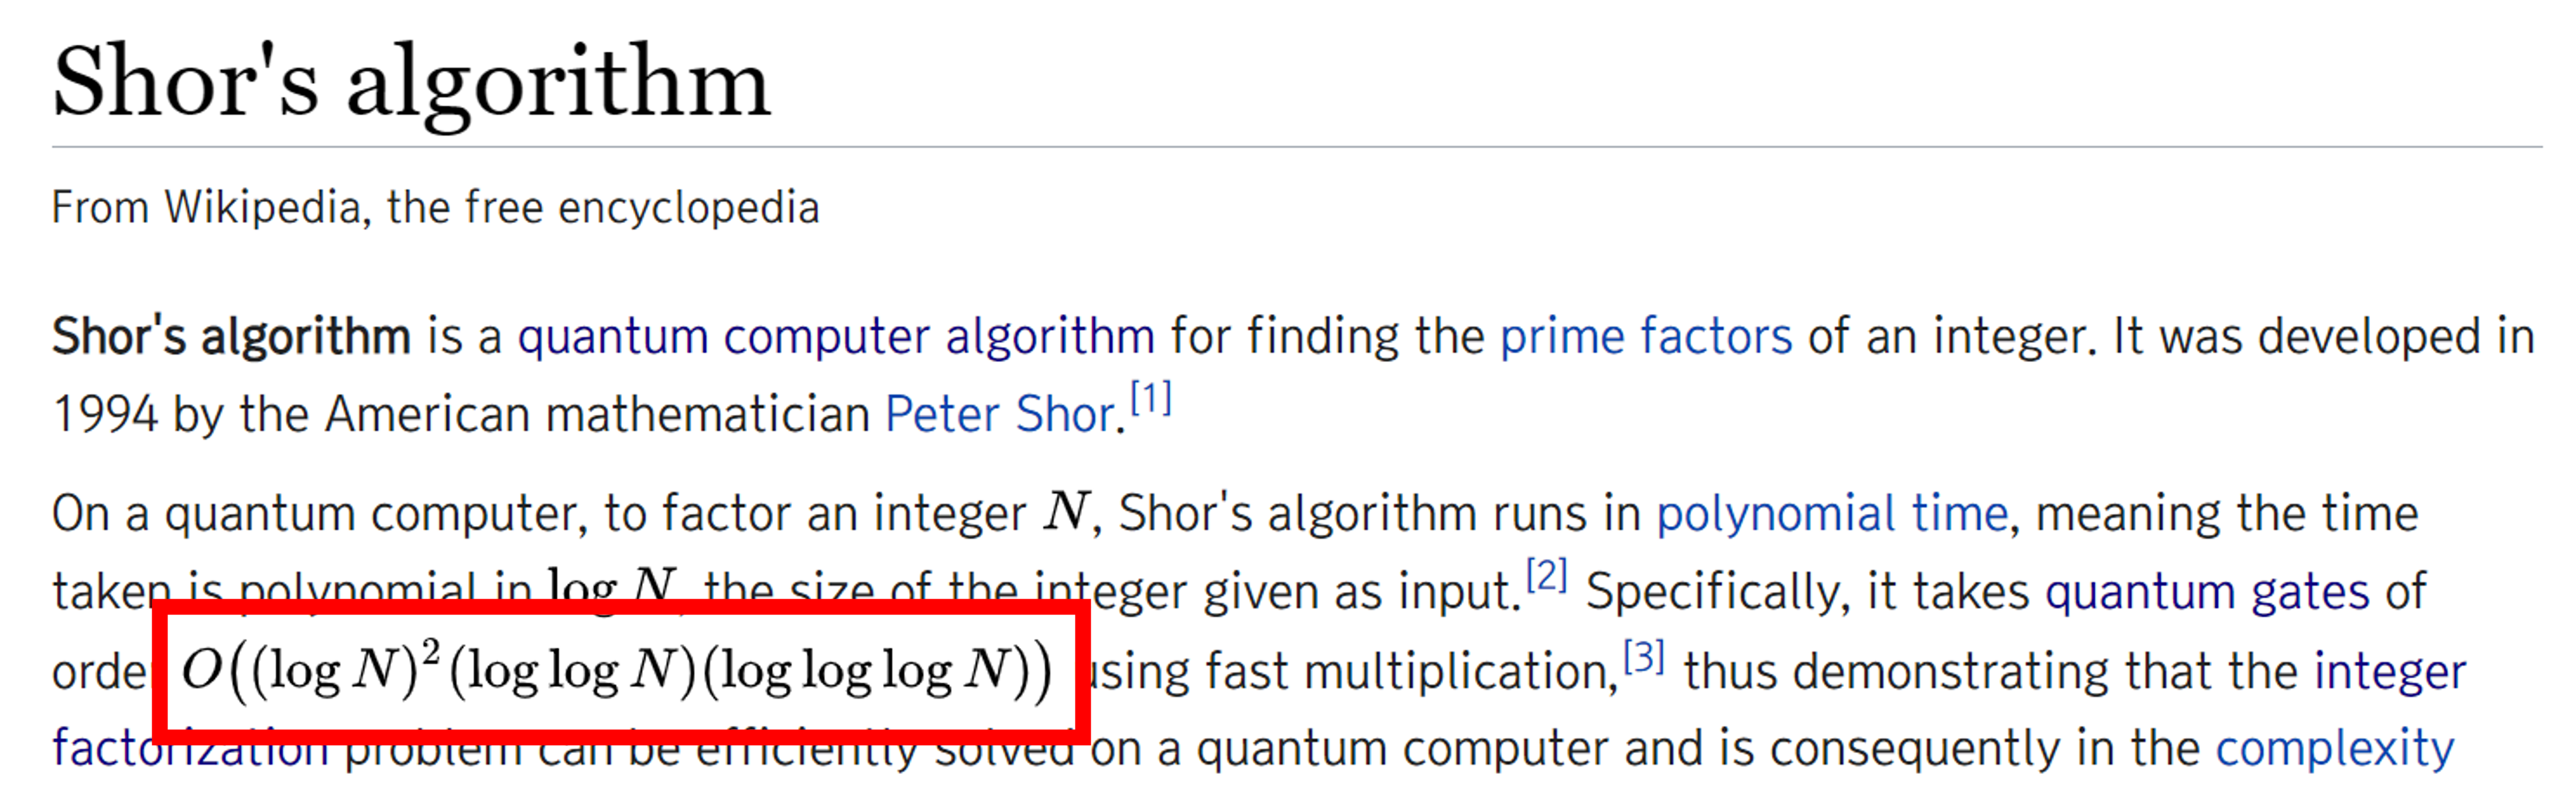
\includegraphics[width=\linewidth]{shor_wikipedia.png}
        \end{figure}
        \footnotesize \vspace*{-1em}
        \centerline{Waiting for this to be updated to $O\big( (\log N)^2 (\log \log N) \big)$ . . .}
    \end{frame}

    \subsection{Quantum Part - Quantum Fourier Transform}
    \begin{frame}{Quantum Fourier Transform}
        \begin{block}{Quantum Fourier Transform (QFT)}
            The \alert{quantum Fourier transform} is a linear transform that maps a basis vector $\vert a \rangle$ as
            \[ \vert a \rangle \mapsto \frac{1}{\sqrt{N}} \sum_{c=0}^{N-1} \omega_N^{ac} \vert c \rangle \]
            where $N$ is the dimension of the vector space and $\omega_N \triangleq e^{2\pi i / N}$. \\[.5em]
            Note that the quantum Fourier transform is equivalent to multiplying a unitary matrix $A_N$.
            \[ \mrm{QFT}\left( \sum_{a=0}^{N-1} x_a \vert a \rangle \right) = \frac{1}{\sqrt{N}} \sum_{a=0}^{N-1} x_a \sum_{c=0}^{N-1} \omega_N^{ac} \vert c \rangle \]
        \end{block}
        \begin{alertblock}{}
            We will now show that QFT can be done with a polynomially many numbers of local quantum gates even if $N$ is exponential.
        \end{alertblock}
    \end{frame}

    \begin{frame}{Constructing a Quantum Gate Array for QFT}
        \begin{block}{Constructing a Quantum Gate Array for QFT}
            Take $N = 2^\ell$ and let us represent an integer $0 \leq a < N$ in binary as $\vert a_{\ell-1} a_{\ell-2} \cdots a_0 \rangle$.
            We need only two types of gates: $R_j$ and $S_{j,k}$.\\[.4em]
            $R_j \in \mrm{Mat}_{N \times N}(\mbb{C})$ acts on the $j^\text{th}$ bit. \\[-.5em] \small
            \begin{table}
                \centering
                \begin{tabular}{rccc}
                           &                                        & $\vert 0 \rangle$ & $\vert 1 \rangle$                  \\
                    $R_j=$ & \multicolumn{1}{c|}{$\vert 0 \rangle$} & $1/\sqrt{2}$      & \multicolumn{1}{c|}{$1/\sqrt{2}$}  \\
                           & \multicolumn{1}{c|}{$\vert 1 \rangle$} & $1/\sqrt{2}$      & \multicolumn{1}{c|}{$-1/\sqrt{2}$}
                \end{tabular}
            \end{table} \vspace*{-.5em} \normalsize
            $S_{j,k} \in \mrm{Mat}_{N \times N}(\mbb{C})$ acts on the $j^\text{th}$ and $k^\text{th}$ bits.\\[-.5em] \small
            \begin{table}
                \centering
                \begin{tabular}{rccccc}
                               &                                         & $\vert 00 \rangle$ & $\vert 01 \rangle$ & $\vert 10 \rangle$ & $\vert 11 \rangle$                        \\
                               & \multicolumn{1}{c|}{$\vert 00 \rangle$} & 1                  & 0                  & 0                  & \multicolumn{1}{c|}{0}                    \\
                    $S_{j,k}=$ & \multicolumn{1}{c|}{$\vert 01 \rangle$} & 0                  & 1                  & 0                  & \multicolumn{1}{c|}{0}                    \\
                               & \multicolumn{1}{c|}{$\vert 10 \rangle$} & 0                  & 0                  & 1                  & \multicolumn{1}{c|}{0}                    \\
                               & \multicolumn{1}{c|}{$\vert 11 \rangle$} & 0                  & 0                  & 0                  & \multicolumn{1}{c|}{$e^{i \theta_{k-j}}$}
                \end{tabular}
            \end{table}\vspace*{-.5em} \normalsize
            where $\theta_{k-j} \triangleq \pi / 2^{k-j}$.
        \end{block}
    \end{frame}

    \begin{frame}{Constructing a Quantum Gate Array for QFT}
        \begin{block}{}
            We apply
            % \[R_{\ell-1}S_{\ell-2,\ell-1}R_{\ell-2}S_{\ell-3,\ell-1}S_{\ell-3,\ell-2}R_{\ell-3}\cdots R_1 S_{0,\ell-1} \cdots S_{0,1} R_0\]
            \[R_0 S_{0,1} \cdots S_{0,\ell-1} R_1 \cdots R_{\ell-3} S_{\ell-3,\ell-2} S_{\ell-3, \ell-1} R_{\ell-2} S_{\ell-2,\ell-1} R_{\ell-1} \]
            to perform a quantum Fourier transform. This will result in
            \[\vert a \rangle \mapsto \frac{1}{\sqrt{N}}\sum_{c=0}^{N-1} \omega_N^{ac} \vert \overline{c} \rangle\]
            where $\overline{c}$ is the bit reversal of $c$. \\[.5em]
            Later, we may perform a postprocess to recover $c$ from $\overline{c}$.
        \end{block}
        \begin{alertblock}{}
            \centerline{Only $\dfrac{\ell(\ell+1)}{2} \in O\big( (\log N)^2 \big)$ local transformations are used.}
        \end{alertblock}
    \end{frame}

    \begin{frame}{Constructing a Quantum Gate Array for QFT}
        \begin{block}{The Matrices Do Perform QFT}
            We now show
            $\vert a \rangle \mapsto N^{-1/2} \sum_{c=0}^{N-1} \omega_N^{ac} \vert \overline{c} \rangle$
            for each basis vector $\vert a \rangle$. \\[1em]
            We shall focus specifically on going from $\vert a \rangle$ to $\vert b \rangle$.
            Let $a_j$, $b_j$, and $\overline{b}_j$ denote the $j^\text{th}$ bit of $a$, $b$, and $\overline{b}$, respectively. \\[.5em]
            We first confirm that the $1/\sqrt{2}$ factors of the $\ell$ number of $R_j$ matrices multiplies to be $N^{-1/2}$ on the amplitude. \\[.5em]
            Note that, $\pi$ is added to the phase if and only if $a_j = b_j = 1$,
            and $\theta_{k-j}$ is added to the phase if and only if $a_j = b_k = 1$.\\[.5em]
            Therefore, the total phase change is\\[.5em]
            \centerline{$\displaystyle \sum_{0 \leq j < \ell} \pi a_j b_j + \sum_{0 \leq j < k < \ell} \theta_{k-j} a_j b_k$.}
        \end{block}
    \end{frame}

    \begin{frame}{Constructing a Quantum Gate Array for QFT}
        \begin{block}{}
            \vspace*{-1em}
            \begin{flalign*}
                \textstyle \sum_{0 \leq j < \ell} & \textstyle \pi a_j b_j + \sum_{0 \leq j < k < \ell} \dfrac{\pi}{2^{k-j}} a_j b_k \\
                &= \textstyle\sum_{0 \leq j \leq k < \ell} \dfrac{\pi}{2^{k-j}} a_j b_k \\
                &= \textstyle\sum_{0 \leq j \leq k < \ell} \dfrac{\pi}{2^{k-j}} a_j \overline{b}_{\ell-k-1} \\
                &= \textstyle\sum_{0 \leq j+k' < \ell} 2\pi \dfrac{2^j 2^{k'}}{2^\ell} a_j \overline{b}_{k'} & \mcomment{Substitute $k' \to \ell-k-1$} \\
                &\equiv_{2\pi} \textstyle\sum_{0 \leq j,k' < \ell} 2\pi \dfrac{2^j 2^{k'}}{2^\ell} a_j \overline{b}_{k'} & \mcomment{No effects on adding $2\pi$s} \\
                &= \textstyle\dfrac{2\pi}{2^\ell} \sum_{j=0}^{\ell-1} 2^j a_j \sum_{k'=0}^{\ell-1} 2^{k'} \overline{b}_{k'} \\
                &= 2\pi a \overline{b} / N
            \end{flalign*}
        \end{block}
    \end{frame}

    \begin{frame}{Constructing a Quantum Gate Array for QFT}
        \begin{block}{}
            Therefore, we got \\[.5em]
            \centerline{$\displaystyle \vert a \rangle \mapsto \frac{1}{\sqrt{N}} \sum_{b=0}^{N-1} e^{2\pi ia\overline{b}/N} \vert b \rangle = \frac{1}{\sqrt{N}} \sum_{b=0}^{N-1} \omega_N^{a\overline{b}} \vert b \rangle\text{,}$} \vspace*{.5em}
            and it is immediate that \\[.5em]
            \centerline{$\displaystyle \vert a \rangle \mapsto \frac{1}{\sqrt{N}} \sum_{c=0}^{N-1} \omega_N^{ac} \vert \overline{c} \rangle$} \vspace*{.5em}
            since $\overline{\,\cdot\,}$ is indeed bijective. \\[.5em]
            With the postprocess\footnote{i.e. reversing the bits after observing}, we may get the same result as having \\[.5em]
            \centerline{$\displaystyle \vert a \rangle \mapsto \frac{1}{\sqrt{N}} \sum_{c=0}^{N-1} \omega_N^{ac} \vert c \rangle\text{.}$}
        \end{block}
    \end{frame}

    \begin{frame}{Approximate Quantum Fourier Transform}
        \begin{block}{Approximate QFT ($\mrm{AQFT}_m$) (Coppersmith; 1994) \href{https://arxiv.org/abs/quant-ph/0201067}{\beamergotobutton{Paper}}}
            If $k-j$ is too large, $\theta_{k-j} = \pi / 2^{k-j}$ gets too small and we end up multiplying a very small phase factor;
            it would be very difficult to do accurately physically.\\[.5em]
            Parametrized by $m \in [\ell]$, the $\mrm{AQFT}_m$ ignores $S_{k-j}$ if $k-j \geq m$.
            Therefore, the total phase change is
            $\sum_{\ell-m \leq j+k' < \ell} 2\pi \dfrac{2^j 2^{k'}}{2^\ell} a_j \overline{b}_{k'}$\footnote{Follow the procedure in the previous page.}.
            The difference is $\sum_{0 \leq j+k' < \ell-m} 2\pi \dfrac{2^j 2^{k'}}{2^\ell} a_j \overline{b}_{k'}$,
            which is bounded by $2\pi \ell 2^{-m}$.
        \end{block}
    \end{frame}

    \subsection{Quantum Part - From Initialization to Observation}
    \begin{frame}{From Initialization to Observation}
        \begin{block}{1. Calculate the Modular Exponentiation}
            \small
            Find $N=2^\ell$ such that $n^2 \leq N < 2n^2$. \\[.5em]
            We will construct the quantum gate array for calculating $x^a \mod n$
            that fixes $x$ and $n$ and treats $a$ as the only input.
            This is possible since we can construct such array in a polynomial time.\\[.5em]
            Suppose we have the uniformly superpositioned state of two registers\footnote{storage that contains a (possibly) superpositioned $2^\ell$-bit quantum state.}\\[.5em]
            \centerline{$N^{-1/2}\sum_{a=0}^{N-1} \vert a, 0 \rangle$.}\vspace*{.5em}
            Making this is easy, since all we have to do is putting each bit of the first register in the superposition $(\vert 0 \rangle + \vert 1 \rangle)/\sqrt{2}$. \\[.5em]
            We now calculate $x^a \mod n$ via the modular exponentiation algorithm made into a reversible quantum gate array, resulting in \\[.5em]
            \centerline{$N^{-1/2}\sum_{a=0}^{N-1} \vert a, x^a \mod n \rangle$.}
        \end{block}
    \end{frame}

    \begin{frame}{From Initialization to Observation}
        \begin{block}{2. Apply the Quantum Fourier Transform}
            \centerline{$N^{-1/2}\sum_{a=0}^{N-1} \vert a, x^a \mod n \rangle$}\vspace*{.5em}
            Now we apply the QFT on the first register, mapping $\vert a \rangle$ to \\[.5em]
            \centerline{$N^{-1/2}\sum_{c=0}^{N-1} \omega_N^{ac} \vert c \rangle$,}\vspace*{.5em}
            letting us having the state \\[.5em]
            \centerline{$N^{-1} \sum_{a=0}^{N-1} \sum_{c=0}^{N-1} \omega_N^{ac} \vert c, x^a \mod n \rangle$,}\vspace*{.5em}
            Now, we \textit{observe}.
        \end{block}
    \end{frame}
    
    \subsection{Quantum Part - Probability Analysis}
    \begin{frame}{Probability Analysis}
        \begin{block}{Probability of Observing $\vert c, x^k \mod n \rangle$}
            \small
            Let $r = \ord{n} x$. We now calculate the probability that
            our machine ends in a particular state $\vert c, x^k \mod n \rangle$ where we may assume $0 \leq k < r$.
            Summing over all $(a, c)$ to reach the state, we find the probability is \\[.5em] 
            \centerline{\normalsize $\left| N^{-1} \sum_{0 \leq a < N; x^a \equiv_n x^k} \omega_N^{ac} \right|^2$.} \vspace*{.5em}
            Since $x^a \equiv_n x^k$ if and only if $a \equiv_r k$, the probability is equal to \\[.5em] 
            \centerline{\normalsize $\left| N^{-1} \sum_{b=0}^{m-1} \omega_N^{(k+br)c} \right|^2$.} \vspace*{.5em}
            where $m-1 \triangleq \lfloor (N-k-1)/r \rfloor$. Since $\omega_N^{kc}$ is a unit-length constant over the summation, now we have \\[.5em]
            \centerline{\normalsize $\left| N^{-1} \sum_{b=0}^{m-1} \omega_N^{brc} \right|^2$.} \vspace*{.5em}
        \end{block}
    \end{frame}

    \begin{frame}{Probability Analysis}
        \begin{exampleblock}{}
            \small \centering
            For all $\theta \in \mbb{R}$,
            $\begin{aligned}[t]
                \big| 1 - e^{i\theta} \big|^2 &= (1 - \cos \theta)^2 + \sin^2 \theta \\
                &= 2 - 2 \cos \theta = 4 \sin^2 (\theta/2)\text{.}
            \end{aligned}$
        \end{exampleblock}
        \begin{block}{}
            \small
            \centerline{$\begin{aligned}[t]
                \textstyle \left| N^{-1} \sum_{b=0}^{m-1} \omega_N^{brc} \right|^2
                &= \textstyle N^{-2} \left| \dfrac{1 - \omega_N^{mrc}}{1 - \omega_N^{rc}} \right|^2 \\
                &= \textstyle N^{-2} \dfrac{\big| 1 - \omega_N^{mrc} \big|^2}{\big| 1 - \omega_N^{rc} \big|^2}
                 =            N^{-2} \dfrac{\sin^2 (\pi mrc/N)}{\sin^2 (\pi rc/N)}
            \end{aligned}$} \vspace*{.5em}
            if $\omega_N^{rc} \neq 1$; otherwise it is equal to $N^{-2}m^2$. \\[.5em]
            Therefore, the probability equals $N^{-2}f(rc/N)$ where
            $f \colon \mbb{R} \to \mbb{R}$ is defined by $f(x) = \dfrac{\sin^2(\pi mx)}{\sin^2(\pi x)}$ for $x \in \mbb{R} \setminus \mbb{Z}$,
            and $f(x) = m^2$ for $x \in \mbb{Z}$. \\[.5em]
            We now analyze $f(x)$ to find the lower bound of the probability.
        \end{block}
    \end{frame}

    \begin{frame}{Probability Analysis}
        \centerline{\fbox{some facts regarding $m = \left\lfloor (N-k-1)/r \right\rfloor$}}
        \begin{exampleblock}{}
            \small \centering
            $\displaystyle m=\left\lfloor \frac{N-k-1}{r} \right\rfloor + 1 > \frac{N-k-1}{r} \geq \frac{N}{r}-1 \geq \left\lfloor \frac{N}{r} \right\rfloor - 1$
        \end{exampleblock}
        \begin{exampleblock}{}
            \small \centering
            $\begin{aligned}[t]
                \frac{rm}{2N} &= \frac{r}{2N} \left( \left\lfloor \frac{N-k-1}{r} \right\rfloor + 1 \right) \leq \frac{N+r-k-1}{2N} \leq \frac{N+r-1}{2N}
            \end{aligned}$ \vspace*{.5em}
            $\begin{aligned}[t]
                \frac{rm}{2N} &= \frac{r}{2N} \left( \left\lfloor \frac{N-k-1}{r} \right\rfloor + 1 \right) > \frac{N-k-1}{2N} \geq \frac{N-r}{2N}
            \end{aligned}$ \vspace*{.5em}
            $\displaystyle \sin^2\left( \frac{\pi rm}{2N} \right) > \sin^2 \left( \frac{\pi}{2} \frac{N-r}{N} \right) = \cos^2 \left( \frac{\pi r}{2N} \right)$
        \end{exampleblock}
        \begin{exampleblock}{}
            \small
            \centerline{$\displaystyle m = \left\lfloor \frac{N-k-1}{r} \right\rfloor + 1 \leq 2 \left\lfloor \frac{N-k-1}{r} \right\rfloor \leq 2 \left\lfloor \frac{N}{r} \right\rfloor \leq \frac{2N}{r}$} \vspace*{.5em}
            Therefore, $r/(2N) \leq 1/m$.
        \end{exampleblock}
    \end{frame}

    \begin{frame}{Probability Analysis}
        \centerline{Let $\lfloor x \rceil \triangleq \min \mrm{argmin}_{n \in \mbb{Z}} |x - n|$.\footnote{i.e., the closest integer to $x$; choose the least if $x$ is a half integer.}}
        \begin{block}{}
            \small
            With some calculation involving derivatives, we get \\[.5em]
            \centerline{$0 < x < 1/m \:\Longrightarrow\: f'(x) < 0$.} \vspace*{.5em}
            Also because of $f$ being an even function, we conclude that \\[.5em]
            \centerline{$|x| \leq \dfrac{r}{2N} \:\Longrightarrow\: f(x) \geq f\left( \dfrac{r}{2N} \right) = \dfrac{\sin^2(\pi mr/2N)}{\sin^2(\pi r / 2N)} > \cot^2(\dfrac{\pi r}{2N}) > \dfrac{4N^2}{\pi^2 r^2}$.} \vspace*{.5em}
            Also, since $1$ is a period of $f$, \ul{given that} $\left| \dfrac{rc}{N} - \left\lfloor \dfrac{rc}{N} \right\rceil \right| \leq \dfrac{r}{2N}$,
            the probability $N^{-2}f(rc/N)$ is greater than \\[.5em]
            \centerline{$\displaystyle \frac{1}{N^2}\frac{4N^2}{\pi^2 r^2} = \frac{4}{\pi^2 r^2} \in \Omega \left( \frac{1}{r^2} \right)$.}
        \end{block}
    \end{frame}

    \begin{frame}{Probability Analysis}
        \begin{block}{When does $\big| rc/N - \lfloor rc/N \rceil \big| \leq r/(2N)$ hold?}
            \small
            $\big| rc/N - \lfloor rc/N \rceil \big| \leq r/(2N)$ holds if and only if 
            the distance between $rc$ and its cloest multiple of $N$ is not greater than $r/2$, or equivalently, \\[.5em]
            \centerline{$\exists d \in \mbb{N},\: |rc-dN| \leq r/2$.} \vspace*{.5em}
            It is also equivalent to \\[.5em]
            \centerline{$\exists d \in \mbb{N},\: \left| \dfrac{c}{N} - \dfrac{d}{r} \right| \leq \dfrac{1}{2N}$.} \vspace*{.5em}
            Since $1/(2N) \leq 1/(2n^2) < 1/(2r^2)$, there exists a unique such reduced fraction $d/r$ with $r < n$,
            and we can obtain it by continued fraction in a polynomial time, by the theorem in \hyperlink{convergent}{\color{blue}this page}.
        \end{block}
    \end{frame}

    \begin{frame}{Probability Analysis}
        \begin{block}{How many values of $\vert c, x^k \mod n \rangle$ would lead us to find the order?}
            \small
            There are $\phi(r)$ values of $d/r$---since $(d, r)$s such that $\gcd(d,r)=1$ will be found by continued fraction---and
            each would lead to a unique value of $c$ because \\[.5em]
            \centerline{$\left| \dfrac{c}{N} - \dfrac{d}{r} \right| \leq \dfrac{1}{2N}$} \vspace*{.em}
            must hold. \\[.5em]
            Also, being independent to the value of $c$, the second register ($x^k \mod n$) may have at most $r$ values. \\[.5em]
            Therefore, we have total $r \phi(r)$ values of $\vert c, x^k \mod n \rangle$ that enable us to find $r$
            using the method mentioned in the last page. \\[.5em]
            In other words, there are $r \phi(r)$ values of $\vert c, x^k \mod n \rangle$ that satisfies $\big| rc/N - \lfloor rc/N \rceil \big| \leq r/(2N)$.
        \end{block}
    \end{frame}

    \begin{frame}{Probability Analysis}
        \begin{block}{Probability of \textit{Observing} a ``Good'' $\vert c, x^k \mod n \rangle$}
            \small
            There are $r \phi(r)$ values of $\vert c, x^k \mod n \rangle$ that satisfies $\big| rc/N - \lfloor rc/N \rceil \big| \leq r/(2N)$, i.e. \textit{good} values. \\[.5em]
            Moreover, as we previously showed, each of those good values has a probability of $\Omega(1/r^2)$. \\[.5em]
            So the total probability is \\[.5em]
            \centerline{$\displaystyle r \phi(r) \cdot \Omega\left( \frac{1}{r^2} \right) = \Omega\left( \frac{\phi(r)}{r} \right) \hyperlink{phigrowth}{\color{blue}=} \Omega\left( \frac{1}{\log \log r} \right)$.} \vspace*{.5em}
            Thus, we need $O(\log \ell)$ number of observations to get a good $\vert c, x^k \mod n \rangle$.
        \end{block}
    \end{frame}

    \begin{frame}{Optimization Methods}
        \begin{block}{Optimization Methods}
            \small
            Since quantum observations seem to be much more expensive than classical computation methods,
            we shall minimize the expected number of observations needed to find $r$.
            \begin{enumerate}
                \item $c \pm 1, c \pm 2, \cdots$ are good candidates if $c$ is observed.
                \item The algorithm does not consider if $r$ shares a common factor with $d$. If they do, the common factor is likely to be small.
                      With considering first $(\log n)^{1+\varepsilon}$ multiples of $r'$ calculated from continued fraction, we may reduce the expected number of observing from $O(\log \ell)$ down to $O(1)$. (Odylzko; 1995)
                \item If two candidates of $r$---$r_1$ and $r_2$---are found through a few observations, $\mrm{lcm}(r_1, r_2)$ is a good candidate. This also reduce the expected number to $O(1)$. (Knill; 1995)\footnote{These results are introduced in the paper as a part of ``conversation''. . .}
            \end{enumerate}
        \end{block}
    \end{frame}

\end{document}